%!TeX program = xelatex
% VizDOM - arc42 Architecture Documentation (English). Compile with XeLaTeX (see README.md).
% Overleaf: Menu -> Settings -> Compiler -> XeLaTeX (fontspec needs XeTeX/LuaTeX).
\documentclass[11pt,a4paper]{report}

\usepackage{fontspec}
\usepackage[english]{babel}
\usepackage{microtype}
\usepackage{geometry}
\geometry{margin=2.4cm}
\usepackage{graphicx}
\usepackage{booktabs}
\usepackage{array}
\usepackage{longtable}
\usepackage{caption}
\usepackage{enumitem}
\usepackage{xcolor}
\usepackage[hidelinks]{hyperref}
\usepackage{float}
\usepackage{titlesec}

\graphicspath{{figures/}}
\newcommand{\code}[1]{\texttt{#1}}
\newcommand{\req}[1]{\textbf{#1}}
\setlength{\parskip}{0.4em}
\setlength{\parindent}{0pt}
\setlength{\tabcolsep}{4pt}
\renewcommand{\arraystretch}{1.25}

% arc42 sections are chapters; keep numbering "N".
\titleformat{\chapter}[hang]{\normalfont\huge\bfseries}{\thechapter}{1em}{}
\titlespacing*{\chapter}{0pt}{0pt}{1em}

\title{\textbf{VizDOM --- Architecture Documentation}\\[0.3em]
\large arc42 template}
\author{Nguyen Huynh Tri Cuong\\
\small Master's Applied Project (Computer Science) --- Ho Chi Minh City University of Science\\
\small Faculty of Information Technology\\
\small Supervisor: Assoc.\ Prof.\ Dr.\ Nguyen Van Vu}
\date{2026 --- Revision 1.0}

\begin{document}
\maketitle

\begin{abstract}
\noindent This document describes the software architecture of \textbf{VizDOM}, a
system that reconstructs a UI-Automator-like Document Object Model (DOM) from a GUI
screenshot to enable test automation of applications that expose no accessibility
tree. It follows the arc42 template and the SWA decision discipline
(drivers~$\rightarrow$~solution~$\rightarrow$~documentation~$\rightarrow$~verification).
The governing principle is traceability: every architecturally significant choice is
linked to a ranked driver and, where possible, to measurable evidence. VizDOM is a
Method-3 applied project; the architecture emphasises modifiability (pluggable
detection/capture/actuation), deployability (each concern runnable locally or as a
remote gRPC service), and testability, over algorithmic novelty.
\end{abstract}

\tableofcontents

% =====================================================================
\chapter{Introduction and Goals}
% =====================================================================
VizDOM converts a GUI \emph{screenshot} into a structured, queryable
\emph{Visual DOM} --- element bounds, roles, text, labels, locators, and
hierarchy --- using computer vision plus a small language/vision model, and exposes
that DOM to a test framework. It targets applications where the platform
accessibility tree (Android UI~Automator, Windows~UIA, the web DOM) is absent or
untrustworthy: custom-rendered desktop UIs (Qt/QML, OpenGL, game engines), embedded
and industrial HMIs, and screens observed through a camera. Where an accessibility
tree exists, frameworks such as Appium build on it~\cite{uiautomator,appium}; VizDOM
targets the cases where it does not.

\paragraph{Problem context.} Detecting GUI elements is harder than natural-image
object detection: at the element level one class varies widely (intra-class
variation) while different classes look alike (inter-class similarity); at the GUI
level widgets, images and text mix, elements are densely packed, and testing needs
high-precision boxes rather than a loose region~\cite{xie2020uied}. No single
detector family --- classical or deep --- is uniformly best across these conditions.
This is the architectural force behind the pluggable detector decision (ADR-015) and
the clean-up stages; the project report treats the full problem/solution space.

\section{Requirements overview}
\subsection*{Functional requirements}
\begin{longtable}{@{}p{1.6cm}p{12.6cm}@{}}
\toprule
\textbf{ID} & \textbf{Functional requirement} \\
\midrule
\endhead
FR1 & Acquire a screenshot from a configurable source (OS desktop, Android device, camera, remote service, or file). \\
FR2 & Detect UI elements and text in a screenshot using a selectable detector backend. \\
FR3 & Assemble detections into a hierarchy and compile a UI-Automator-like DOM (roles, flags, labels, multiple locators). \\
FR4 & Resolve a locator (by id/text/hint/role/spatial relation) to a concrete element. \\
FR5 & Drive input (click, type, key, scroll, drag) against a resolved element. \\
FR6 & Expose the above to Robot Framework as keywords. \\
FR7 & Allow capture, detection, and actuation to run as remote services across machines/devices. \\
FR8 & Allow users to add new detector/capture/actuator backends without modifying the core. \\
\bottomrule
\end{longtable}

\subsection*{Quality requirements (measurable)}
\begin{longtable}{@{}p{1.6cm}p{4.0cm}p{8.6cm}@{}}
\toprule
\textbf{ID} & \textbf{Quality} & \textbf{Measurable statement} \\
\midrule
\endhead
NFR1 & Modifiability & A new detector/capture/actuator backend is added by adding one file and a registry entry, with \textbf{zero} edits to the domain core; each port has $\geq 2$ interchangeable implementations. \\
NFR2 & Deployability & Each port is selectable as \emph{in-process} or \emph{gRPC} purely by configuration; a capture$\rightarrow$detect$\rightarrow$actuate flow runs unchanged across $\geq 2$ hosts. \\
NFR3 & Performance & A detector service loads its model \textbf{once} (warm model) and serves subsequent requests without reloading; per-request latency excludes model-load time. \\
NFR4 & Testability & The domain core runs end-to-end with no GPU and no network (UIED detector + static-image capture + recording actuator). \\
NFR5 & Accuracy & Target: element detection F1 $\geq 0.80$ and mean IoU $\geq 0.60$ on a labelled benchmark. Measured (44-image synthetic set): aggregate F1 $0.58$ (OmniParser) / $0.51$ (UIED), mIoU 0.67--0.68 --- mIoU target met, F1 target \emph{not} met. Per-type, OmniParser leads on actionable controls (button 1.00, input\_field 0.99, icon 0.67) and UIED on checkbox/text; both are click-targetable (center-hit: OmniParser actionable 0.97, UIED 0.89). See Ch.~10--11. \\
\bottomrule
\end{longtable}

\section{Quality goals (top 3)}
\begin{enumerate}[leftmargin=1.6em]
  \item \req{Modifiability / extensibility} --- swapping and adding backends is the
        central design intent; the value of the system is that classical and learned
        detectors, and diverse capture/actuation devices, are interchangeable.
  \item \req{Deployability} --- capture runs where the app-under-test is, detection
        benefits from a GPU, actuation happens at the device or a physical
        controller; the architecture must let these live on different machines.
  \item \req{Testability} --- the pipeline and the Robot Framework layer must be
        verifiable without special hardware, so the project can be developed and
        graded on a laptop.
\end{enumerate}

\section{Stakeholders}
\begin{longtable}{@{}p{3.4cm}p{2.2cm}p{2.0cm}p{6.0cm}@{}}
\toprule
\textbf{Stakeholder} & \textbf{Interest} & \textbf{Power} & \textbf{Primary need} \\
\midrule
\endhead
Student / author & High & High & A working, defensible applied system and report. \\
Supervisor / examiner & High & High & Clear engineering, traceable decisions, honest evaluation. \\
Test engineers (users) & High & Low & Reliable element location on non-accessible UIs; simple keywords. \\
Device/robotics integrators & Medium & Low & A seam to plug in cameras / robot arms. \\
Operations (future) & Low & Low & Services that start, log, and fail safely. \\
\bottomrule
\end{longtable}

% =====================================================================
\chapter{Architecture Constraints}
% =====================================================================
\begin{longtable}{@{}p{3.6cm}p{11.0cm}@{}}
\toprule
\textbf{Constraint} & \textbf{Detail and consequence} \\
\midrule
\endhead
Runtime & Python 3.9 with a CUDA-enabled PyTorch (cu124) build; the working interpreter must not be disturbed by environment tooling. \\
Environment manager & \code{uv} is used over the existing interpreter (no re-provisioning of the working CUDA build). \\
Corporate proxy & Public code hosts (GitHub, Maven) are blocked; PyPI and the PyTorch index are reachable. External model code is \emph{vendored and pinned by a setup script}, not a git submodule; documentation renders UML \emph{offline} from a local renderer. \\
No container runtime & Docker/Nomad/Consul are explicitly excluded (resource cost); distribution uses plain gRPC processes and launcher scripts. \\
Dependency pin & \code{protobuf < 6} project-wide (Streamlit/TensorFlow conflict); \code{grpcio}/\code{grpcio-tools} pinned accordingly. \\
Licensing & OmniParser's icon detector is AGPL-3.0 (via Ultralytics); network-serving that backend carries AGPL obligations. UIED remains an AGPL-free CPU baseline. \\
Diagrams & PlantUML sources are ASCII-only and render via a vendored jar (Smetana layout; \code{architecture.puml} uses Graphviz). \\
Project type & Method-3 applied project: solid engineering with scientific content, not a novel-algorithm thesis. \\
\bottomrule
\end{longtable}

% =====================================================================
\chapter{Context and Scope}
% =====================================================================
\section{Business context}
VizDOM sits between a \emph{screen} (the application under test) and a \emph{test
framework}. Its inbound interface is an image; its outbound interface is a DOM plus
the ability to actuate input. Figure~\ref{fig:overview} shows the end-to-end flow.

\begin{figure}[H]
  \centering
  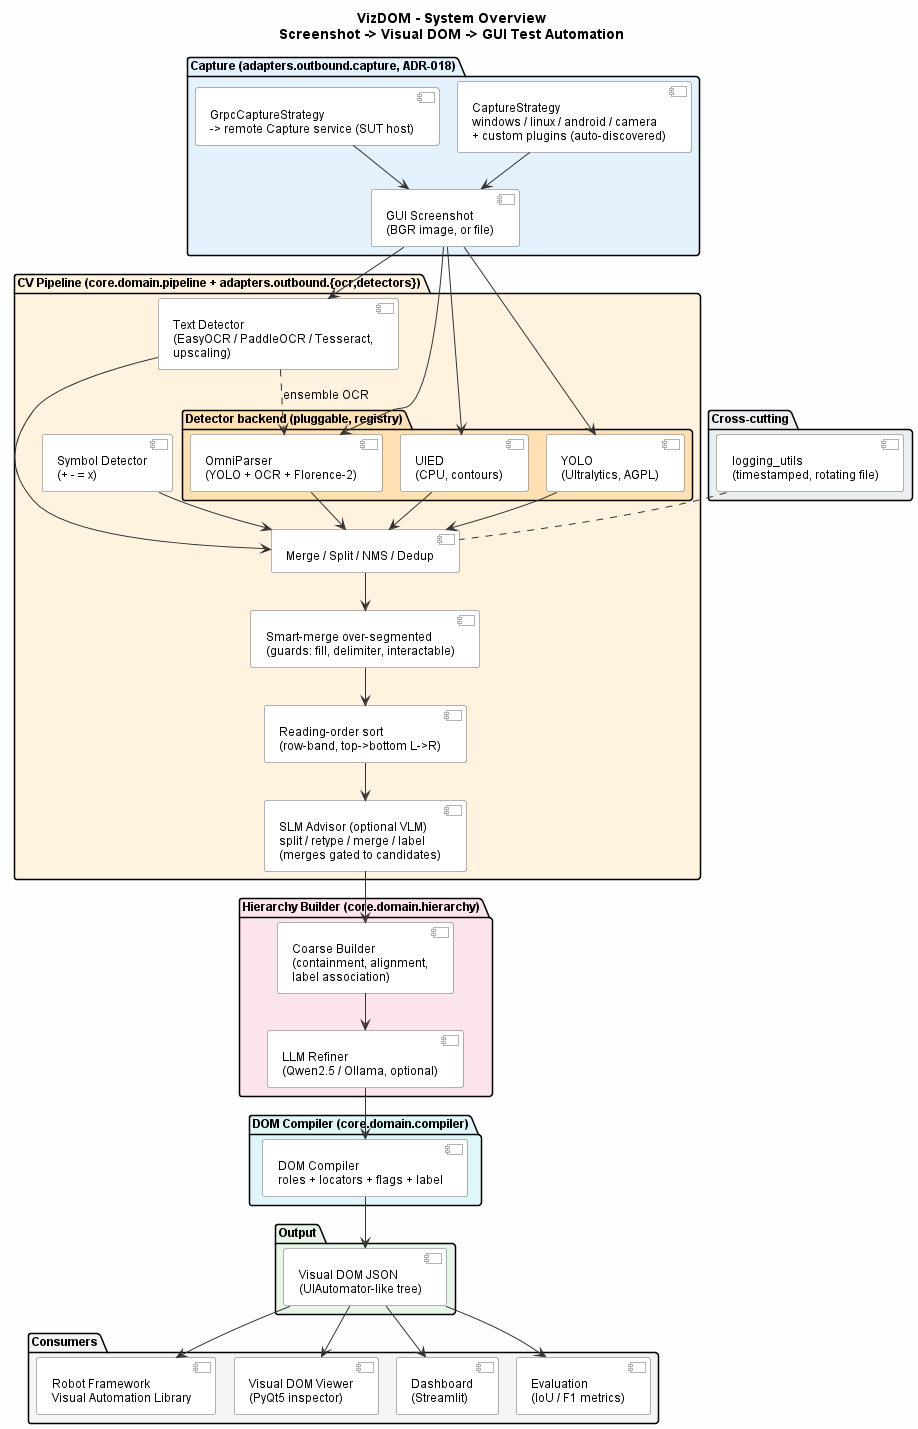
\includegraphics[width=0.6\linewidth]{System_Overview.png}
  \caption{System overview / context. Left boundary: a screenshot from any capture
  source. Right boundary: a Visual DOM consumed by Robot Framework, the Viewer, the
  dashboard, and the evaluation harness. Legend: coloured packages are subsystems;
  arrows are data/control flow.}
  \label{fig:overview}
\end{figure}

\section{Technical context (interfaces)}
\begin{longtable}{@{}p{3.4cm}p{3.0cm}p{7.6cm}@{}}
\toprule
\textbf{Neighbour} & \textbf{Direction} & \textbf{Interface} \\
\midrule
\endhead
App under test & inbound & Screenshot (BGR image) via a capture strategy; input events via an actuator strategy. Optionally \emph{raised to the foreground} first (window title / Android activity), since a whole-screen grab and coordinate-based input both silently target the wrong application otherwise (ADR-021). \\
OCR engines & outbound & EasyOCR~\cite{easyocr} / PaddleOCR / Tesseract~\cite{tesseract} (in-process libraries). \\
OmniParser & outbound & Vendored repo~\cite{omniparser2024} + Florence-2~\cite{florence2} / YOLO~\cite{ultralytics} weights (local files). \\
Ollama & outbound & HTTP to a local/remote small LM/VLM for optional refinement. \\
Remote services & both & gRPC~\cite{grpc}: detector (\code{:50051}), capture (\code{:50053}), actuator (\code{:50054}). \\
Robot Framework & inbound & Keyword library (Python)~\cite{robotframework} consuming the DOM. \\
\bottomrule
\end{longtable}

\section{Scope}
\textbf{In scope:} screenshot acquisition, element/text detection, DOM synthesis,
locator resolution, input actuation, the Robot Framework library, and the
distributed service transport. \textbf{Out of scope:} test-case authoring and
scheduling (left to Robot Framework), a hosted multi-tenant service, authentication
of the gRPC channels (flagged as debt), and any modification of the applications
under test.

% =====================================================================
\chapter{Solution Strategy}
% =====================================================================
\section{Strategy summary}
\begin{longtable}{@{}p{3.4cm}p{11.2cm}@{}}
\toprule
\textbf{Quality goal} & \textbf{Architectural approach} \\
\midrule
\endhead
Modifiability & \emph{Hexagonal (ports \& adapters)}: a pure domain core depends only on abstract ports (Detector, Ocr, Refiner, Capture, Actuator). Each port uses a \emph{strategy + registry + auto-discovery} pattern, so backends are added as plugins. \\
Deployability & Each driven port has an in-process adapter \emph{and} a gRPC-client adapter; a matching gRPC server wraps the registry on the remote host. Transport is a per-port configuration choice, not a rewrite. \\
Performance & Model services are \emph{warm}: they load a heavy model once and serve many lightweight clients, amortising load cost. \\
Testability & The core is I/O-free and depends on ports; a dependency-free CPU detector (UIED), a static-image capture, and a recording actuator make full runs possible with no GPU and no network. \\
Accuracy & A pluggable learned detector (OmniParser) plus an OCR ensemble and a guarded small-model refinement stage; classical UIED as a baseline. \\
\bottomrule
\end{longtable}

\section{Ranked drivers}
Context: this is a \emph{greenfield} applied project whose explicit purpose is
extensibility across detectors and devices; modifiability and deployability
therefore rank above raw accuracy. (Were VizDOM a fixed single-platform product,
accuracy and reliability would rank first.)

\begin{longtable}{@{}p{0.8cm}p{2.8cm}p{7.4cm}p{2.4cm}@{}}
\toprule
\textbf{Rank} & \textbf{Driver} & \textbf{Specific interpretation} & \textbf{Type} \\
\midrule
\endhead
\#1 & Modifiability & New detector/capture/actuator without core changes & Requirement \\
\#2 & Deployability & Ports runnable in-process or remote by config & Requirement \\
\#3 & Testability & Full runs with no GPU/network & Requirement \\
\#4 & Accuracy & Detection F1/IoU on real UIs & Requirement \\
\#5 & Performance & Warm-model reuse; acceptable per-request latency & Requirement \\
-- & Offline operation & Proxy blocks public hosts (vendoring, offline docs) & Constraint \\
-- & No containers & Distribution without Docker/Nomad/Consul & Constraint \\
\bottomrule
\end{longtable}

\paragraph{Driver conflicts.}
(a) \emph{Accuracy vs Testability/Portability:} the most accurate detector
(OmniParser) needs a GPU and heavy weights, conflicting with ``runs on a laptop.''
Resolved by making the detector a port with a CPU baseline (UIED) and a remote GPU
service. (b) \emph{Deployability vs Simplicity:} gRPC services add moving parts;
resolved by making gRPC optional (in-process by default).

\section{Key decision: how to make detection/capture/actuation extensible and deployable}
Three alternatives were considered and scored against criteria derived from the
ranked drivers (weights in parentheses): Modifiability~(5), Deployability~(5),
Testability~(4), Complexity~(3, lower is better), Operational complexity~(3, lower
is better). Scores are 1--5.

\begin{longtable}{@{}p{5.2cm}p{1.2cm}p{2.2cm}p{2.2cm}p{2.2cm}@{}}
\toprule
\textbf{Criterion} & \textbf{Wt} & \textbf{A: hard-coded per consumer} & \textbf{B: shared lib, in-process only} & \textbf{C: strategy+registry + optional gRPC} \\
\midrule
\endhead
Modifiability & 5 & 1 (5) & 4 (20) & 5 (25) \\
Deployability & 5 & 1 (5) & 2 (10) & 5 (25) \\
Testability & 4 & 2 (8) & 4 (16) & 5 (20) \\
Complexity (lower better) & 3 & 4 (12) & 4 (12) & 2 (6) \\
Operational (lower better) & 3 & 5 (15) & 4 (12) & 2 (6) \\
\midrule
\textbf{Total} & & \textbf{45} & \textbf{70} & \textbf{82} \\
\bottomrule
\end{longtable}

\textbf{Outcome:} Option~C (chosen). It wins decisively on modifiability and
deployability, the two top drivers, at the cost of higher intrinsic and operational
complexity --- the trade-off we explicitly accept and mitigate by keeping gRPC
optional (Option~B's behaviour is the default local mode) and by sharing one
registry pattern across all three ports. Recorded in ADR-015 (detectors), ADR-017
(distributed gRPC), ADR-018 (capture), ADR-019 (actuator). The decomposition is
deliberately \emph{microservice-oriented}: each port is a first-class service
boundary with a versioned protobuf contract and a standalone server, buying
independent scaling (one warm-GPU detector for many clients), heterogeneous
placement, and fault isolation --- while the same services collapse into one
process when co-location suffices, so distribution is adopted incrementally.
Two later decisions complete the client surface: a single JSON \emph{session
configuration} drives every stage from \code{connect()} or the Robot Framework
\code{Connect} keyword (ADR-020), and a \code{desc=} locator resolves
natural-language element descriptions through a tiered grounding chain ---
deterministic lexical matching first, then a small LM over the DOM, optionally a
vision model via Set-of-Mark --- with positional words enforced geometrically and
per-screen caching (ADR-022).

\section{Detector landscape (why a pluggable port)}
The detector port must accommodate very different technologies. Table~\ref{tab:models}
compares the candidate systems~\cite{xie2020uied,omniparser2024,ariaui2024,elam7b,osworldg}.
They split into two families: \emph{parsers} that enumerate elements (UIED,
OmniParser, VizDOM) and \emph{grounders} that return a single point for a
natural-language instruction (Aria-UI, ELAM-7B, Jedi). Only parsers fit VizDOM's
goal of producing a complete tree; none of the compared systems build a hierarchy,
which is where the contribution sits. The pluggable port lets VizDOM adopt the
strongest parser (OmniParser) as a backend, keep a CPU baseline (UIED) for
GPU-less rigs, and swap an AGPL detector for a permissive one without pipeline
changes --- the concrete justification for ADR-015. The OmniParser backend
additionally maps its coarse \code{text}/\code{icon} output to VizDOM's role
taxonomy (\code{button} / \code{input\_field} / \code{checkbox}) via an
interactivity + resolution-aware geometry heuristic, so its DOM is directly usable
by the test layer. Table~\ref{tab:arc42typeacc} quantifies this mapping: recovering
roles from interactivity, geometry and OmniParser's caption raised element-type
accuracy on actionable controls from \textbf{0.09} to \textbf{0.87}.

\begin{table}[H]
  \centering\footnotesize
  \caption{OmniParser element-type accuracy on matched actionable controls, across
  the two improvement stages (synthetic test set): before (text/icon only), first fix
  (interactivity + geometry), and now (+ caption + re-tuned width/aspect).}
  \label{tab:arc42typeacc}
  \begin{tabular}{@{}lccc@{}}
    \toprule
    GT type & Before & First fix & Now \\
    \midrule
    button       & 0.00 & 0.91 & 0.89 \\
    input\_field & 0.00 & 0.99 & 0.99 \\
    checkbox     & 0.00 & 0.12 & 0.55 \\
    icon         & 1.00$^\dagger$ & 0.00 & \textbf{0.89} \\
    \midrule
    actionable   & 0.09 & 0.73 & \textbf{0.87} \\
    \bottomrule
  \end{tabular}
\end{table}

\noindent{\footnotesize $^\dagger$The old mapping labelled every non-text element
\code{icon}, so only icons scored correct while all other roles scored 0 --- which
is why the DOM could not identify anything actionable. Localisation is unchanged;
this measures \emph{type} only.}

\begin{table}[H]
  \centering\footnotesize
  \caption{The GUI-understanding landscape (author-reported; ``n/v'' = licence not
  yet verified).}
  \label{tab:models}
  \begin{tabular}{@{}p{2.3cm}p{2.4cm}p{2.7cm}p{0.7cm}p{2.2cm}p{2.0cm}@{}}
    \toprule
    System & Paradigm & Output granularity & GPU & Base / size & License \\
    \midrule
    VizDOM (ours) & parser (CV + SLM) & hierarchical DOM tree & No$^\ast$ & composed pipeline & per backend \\
    UIED & classical CV & flat elements & No & --- & research \\
    OmniParser V2 & detector + caption & flat labelled boxes + interactability & Yes & YOLOv8 + Florence-2 & AGPL-3.0 / MIT \\
    Aria-UI & vision grounding & single point $[0,1000]$ & Yes & Aria MoE (3.9B act.) & n/v \\
    ELAM-7B & grounding + eval & point + PASSED/FAILED & Yes & Molmo-7B-D (Qwen2-7B) & Apache-2.0 \\
    Jedi-3B/7B & vision grounding & single point & Yes & 3B / 7B & n/v \\
    \bottomrule
  \end{tabular}\\[0.3em]
  {\footnotesize $^\ast$ CPU via the UIED backend; the OmniParser backend needs a GPU for practical speed.}
\end{table}

% =====================================================================
\chapter{Building Block View}
% =====================================================================
\section{Level 1 --- whitebox VizDOM}
\begin{longtable}{@{}p{3.8cm}p{10.8cm}@{}}
\toprule
\textbf{Building block} & \textbf{Responsibility} \\
\midrule
\endhead
\code{visual\_dom.core.domain} & The hexagon interior (pure, no I/O): pipeline orchestration; hierarchy builder + optional LLM refiner; DOM compiler; schema; reading-order; \code{cvops} (symbol/screen detection, image processing). \\
\code{visual\_dom.core.ports.\allowbreak outbound} & The driven-port interfaces the core depends on: \code{detector\_port}, \code{capture\_port}, \code{actuator\_port}. \\
\code{visual\_dom.adapters.\allowbreak outbound} & Concrete implementations of the ports: \code{detectors} (UIED/YOLO/OmniParser/gRPC + registry), \code{ocr} (text detector), \code{refiner} (SLM advisor), \code{capture} and \code{actuator} (built-ins + gRPC client + user plugins). \\
\code{visual\_dom.adapters.\allowbreak inbound.grpc} & Driving adapters: the detector, capture and actuator gRPC servers. \\
\code{visual\_dom.context} & Composition root --- \code{connect()} / \code{Session} wire adapters to the core from one config. \\
\code{visual\_dom} (config, generated, shared) & \code{config} (VizDomConfig), \code{generated} (protobuf stubs), \code{logging\_utils} (one logger for every component; file + console + Robot-log destinations --- see Ch.~8); \code{evaluation} is a harness outside the hexagon. \\
\code{visual\_gui\_library} & Robot Framework keyword library (thin client over capture + actuator). \\
tools & PyQt5 Viewer, Streamlit dashboard, annotator. \\
\bottomrule
\end{longtable}

\noindent The package tree deliberately mirrors ports \& adapters --- \code{core/}
(domain + ports) inward, \code{adapters/} (inbound + outbound) outward --- so the
layout \emph{is} the architecture. An automated fitness test
(\code{tests/architecture/test\_hexagon.py}) asserts the dependency direction: it
fails if \code{core/} gains a new import of \code{adapters/}. The current, tracked
exceptions are the pipeline directly constructing its OCR/UIED/refiner backends;
they retire when those move behind ports.

\begin{figure}[H]
  \centering
  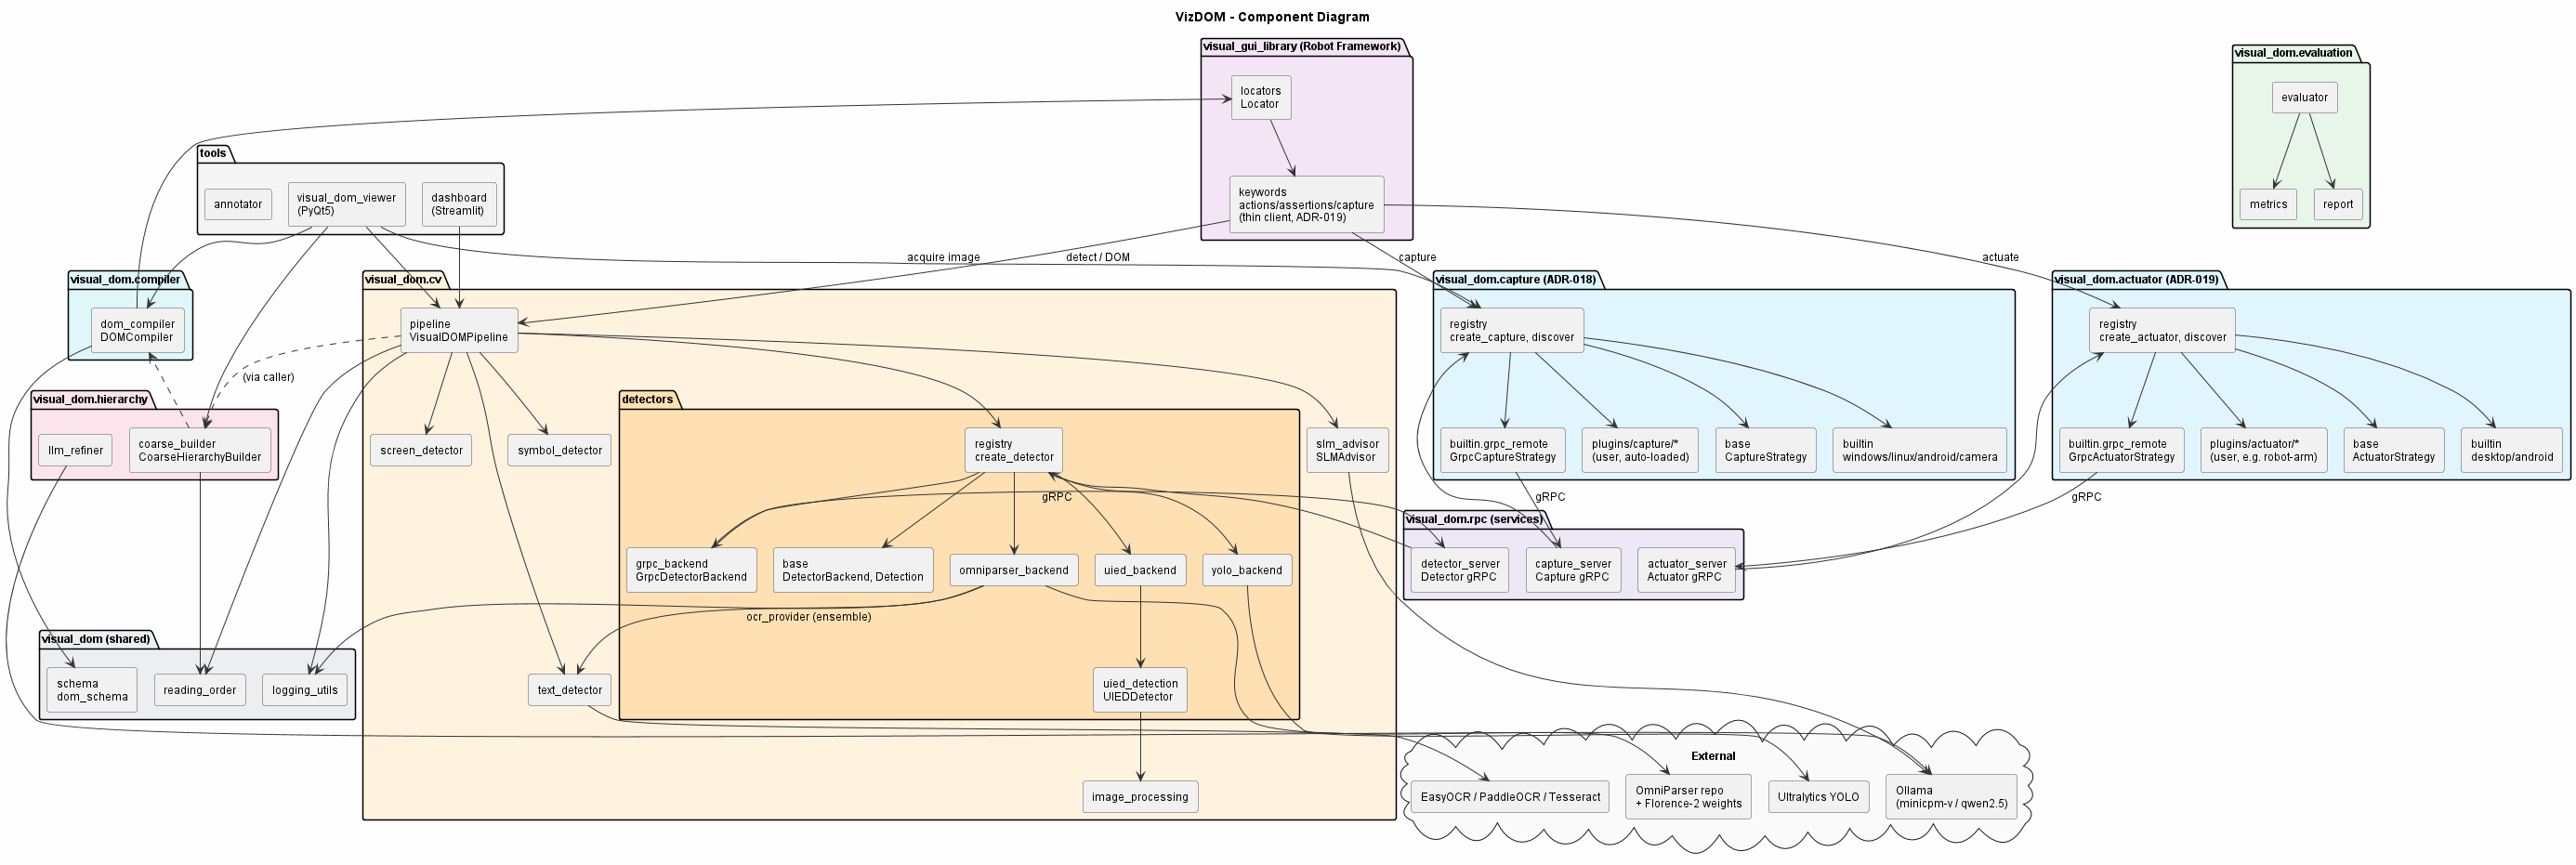
\includegraphics[width=\linewidth]{Component_Diagram.png}
  \caption{Level-1/2 building blocks and dependencies. Legend: coloured boxes are
  packages; nested boxes are subpackages; arrows are ``depends on / calls''. System
  boundary: everything except the \emph{External} cloud (OCR engines, OmniParser
  weights, Ollama, YOLO).}
  \label{fig:component}
\end{figure}

\section{Level 2 --- the driven-port pattern}
Every driven port (detector, capture, actuator) shares the same internal structure:
\begin{itemize}[leftmargin=1.4em]
  \item a \textbf{strategy base} (abstract methods: e.g. \code{detect} /
        \code{capture} / \code{tap+type+swipe});
  \item a \textbf{registry} exposing \code{create\_X(name)}, \code{list\_X()},
        \code{auto\_select()};
  \item \textbf{auto-discovery} that imports built-ins and any user plugin dropped
        in a conventional folder;
  \item a \textbf{gRPC-client strategy} registered under the name \code{grpc}, so a
        remote adapter is selected exactly like a local one.
\end{itemize}
This single pattern, repeated three times, is the mechanism behind NFR1 and NFR2.

\section{Level 2 --- the CV pipeline internals}
The \code{adapters.outbound.detectors} package holds the \code{DetectorBackend}
port implementation set --- a registry factory plus the UIED/YOLO/OmniParser/gRPC
backends; the \code{core.domain.pipeline} additionally owns merge/split/NMS,
smart-merge, reading-order, and the SLM-review stages (Ch.~6).

% =====================================================================
\chapter{Runtime View}
% =====================================================================
\section{Scenario 1 --- local screenshot to DOM (happy path)}
Figure~\ref{fig:seq} shows one cycle with the OmniParser detector and SLM review
enabled. The pipeline detailed flow is in Figure~\ref{fig:pipeline}.

\begin{figure}[H]
  \centering
  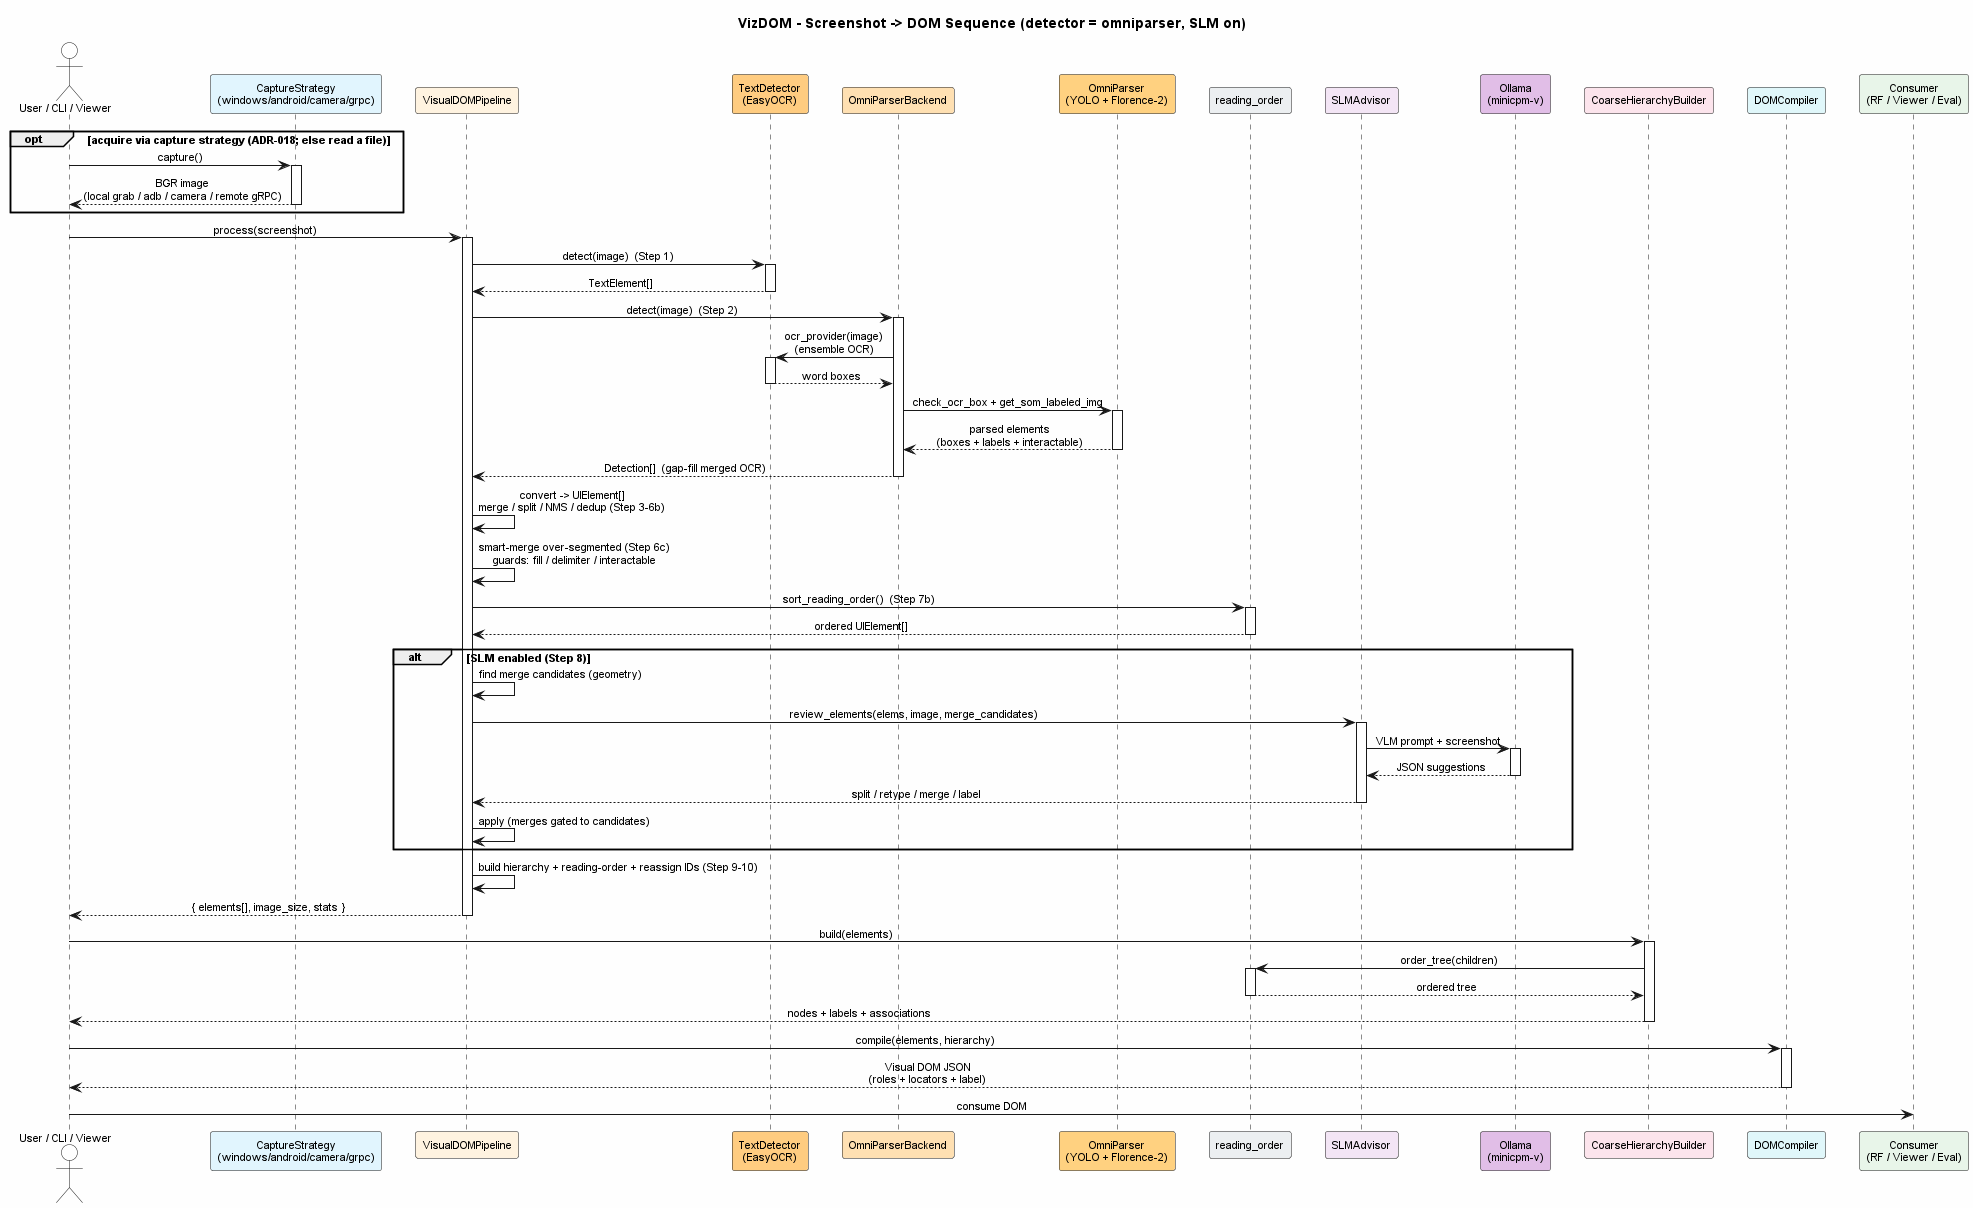
\includegraphics[width=\linewidth]{Sequence_Diagram.png}
  \caption{Runtime scenario 1: capture (optional) $\rightarrow$ OCR $\rightarrow$
  detection with OCR ensemble $\rightarrow$ clean-up $\rightarrow$ reading-order
  $\rightarrow$ optional SLM review $\rightarrow$ hierarchy $\rightarrow$ DOM.}
  \label{fig:seq}
\end{figure}

\begin{figure}[H]
  \centering
  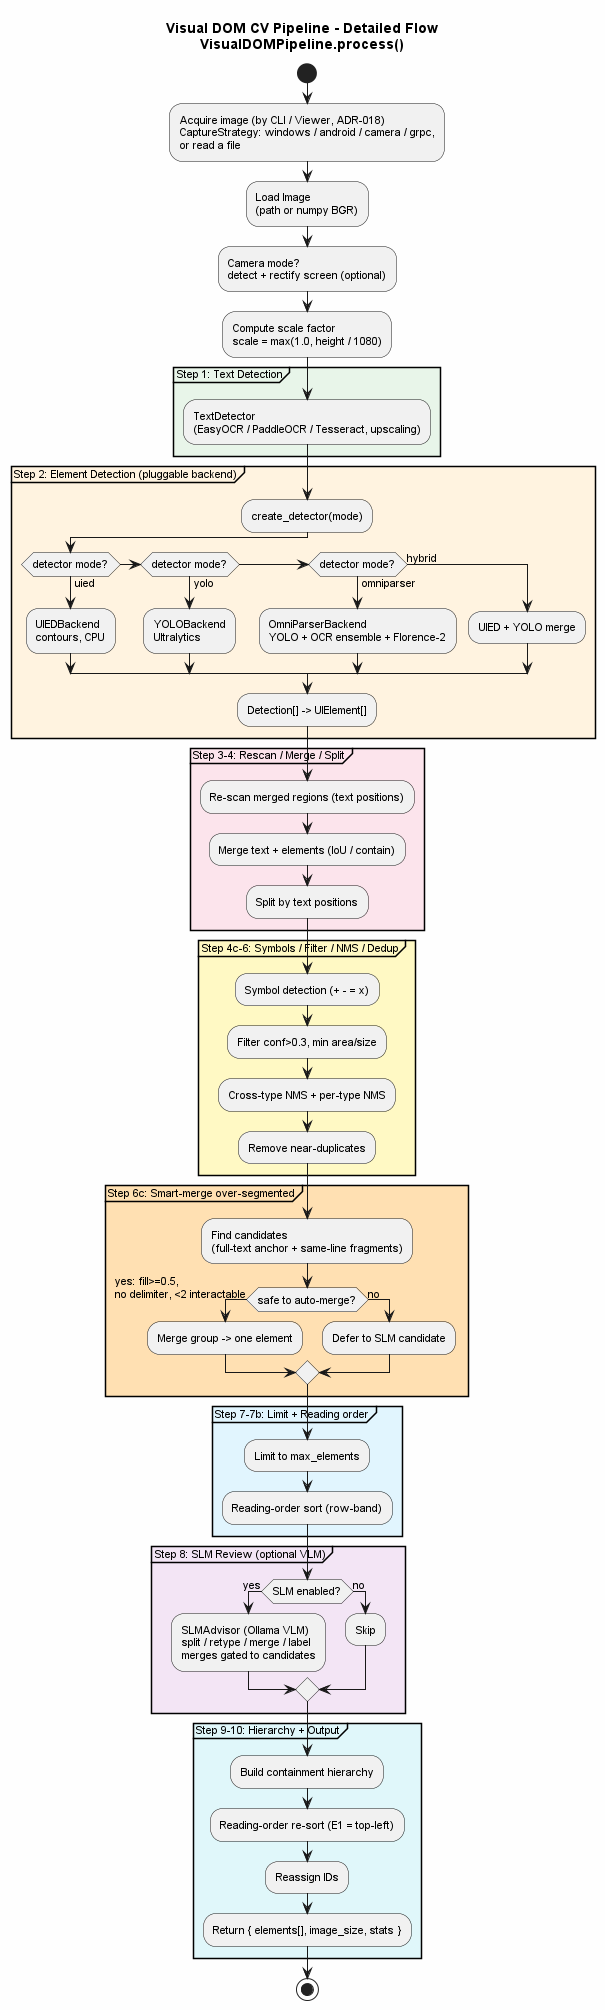
\includegraphics[height=0.82\textheight,width=\linewidth,keepaspectratio]{CV_Pipeline_Detail.png}
  \caption{Runtime scenario 1, detailed control flow of
  \code{VisualDOMPipeline.process()}, including the detector-mode branch and the
  guarded smart-merge / SLM decisions.}
  \label{fig:pipeline}
\end{figure}

\section{Scenario 2 --- distributed capture, detect, actuate}
A test run is orchestrated on a client while: capture runs on the device under test
(\code{grpc} capture $\rightarrow$ capture service), detection runs on a GPU host
(\code{grpc} detector $\rightarrow$ warm-model detector service), and actuation runs
on the device or a robot-arm controller (\code{grpc} actuator $\rightarrow$ actuator
service). Normalised coordinates travel on the actuator wire and are mapped to
device space server-side. Deployment topology is in Figure~\ref{fig:arch}.

\section{Scenario 3 --- failure paths}
\begin{longtable}{@{}p{4.4cm}p{10.2cm}@{}}
\toprule
\textbf{Failure} & \textbf{Designed behaviour} \\
\midrule
\endhead
Remote detector unreachable & The gRPC client call raises; the CLI/Viewer surfaces the error. Mitigation/fallback: select the in-process UIED backend (config change), which needs no GPU or network. \\
Bad image to a service & Servers validate and return an \code{INVALID\_ARGUMENT}/\code{INTERNAL} status with a message; the server process stays up (a single bad request never crashes it). \\
Detector over-segments & Rule-based smart-merge (fill-ratio / delimiter / interactable guards) and the guarded SLM merge correct fragmentation; merges are gated to geometric candidates so distinct controls are never fused. \\
OCR misses text & The OCR ensemble feeds our upscaling OCR into OmniParser to recover missed words (gap-fill dedup). \\
SLM/Ollama unavailable & The refinement stage is optional; the pipeline proceeds with CV results only. \\
\bottomrule
\end{longtable}

% =====================================================================
\chapter{Deployment View}
% =====================================================================
\section{Development / single machine}
All ports run in-process in one Python process; no services are started. This is the
default and the mode used for tests and grading.

\section{Distributed}
\begin{figure}[H]
  \centering
  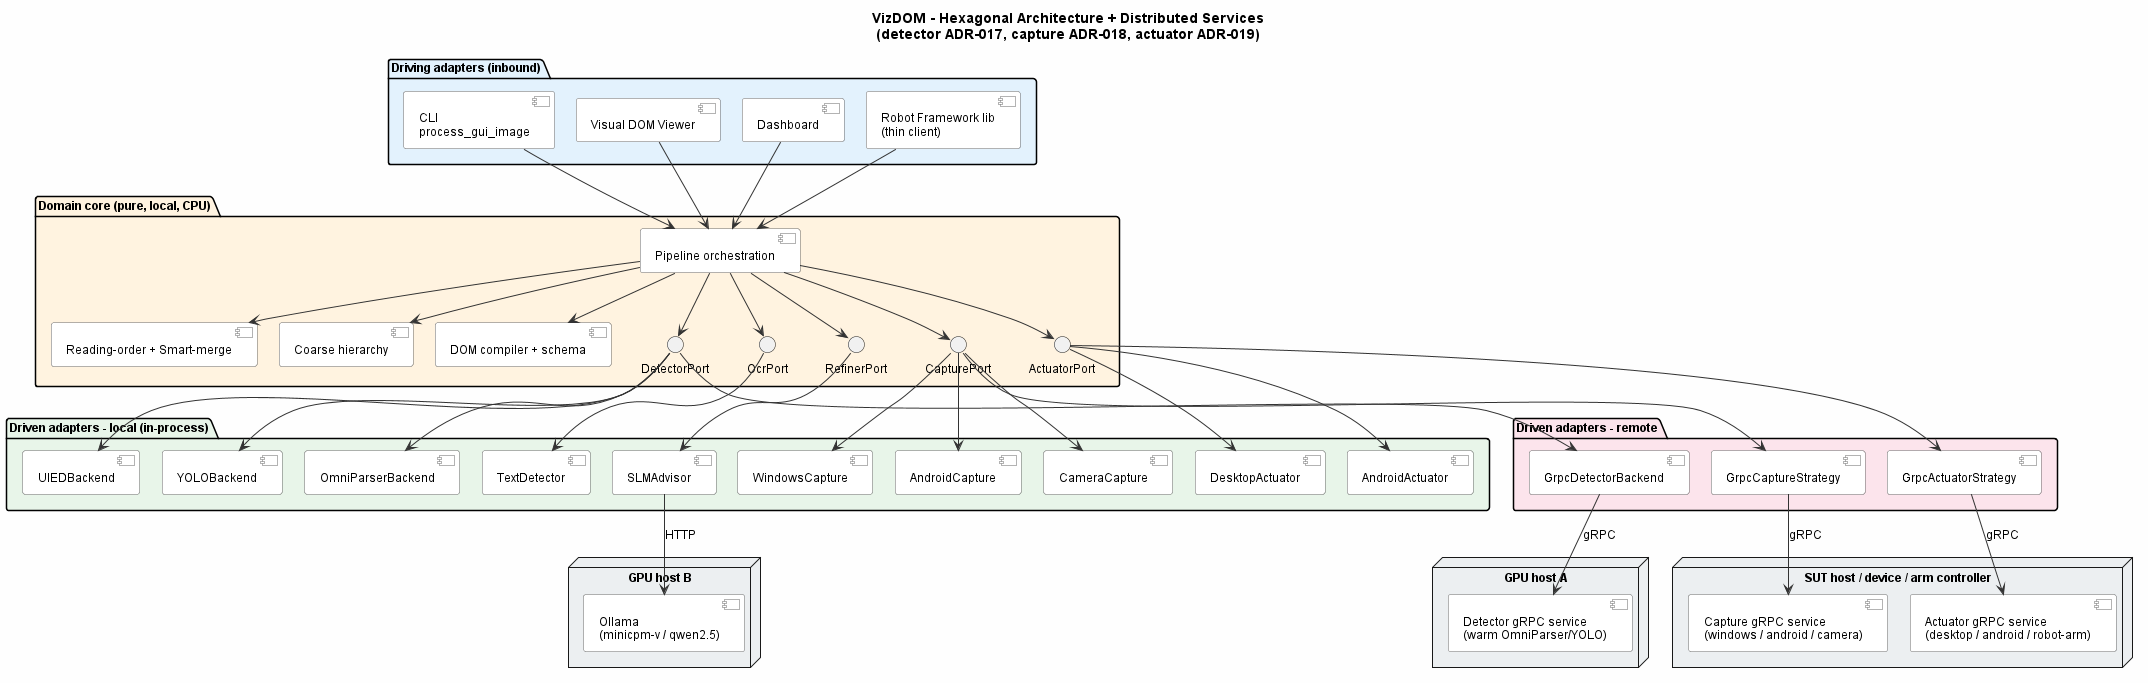
\includegraphics[width=\linewidth]{Architecture.png}
  \caption{Deployment / ports-and-adapters view. Driving adapters (top) enter the
  core; driven ports (middle band) bind to local adapters or remote gRPC adapters;
  the gRPC services run on the GPU host(s) and the SUT/robot-arm controller (bottom).
  Legend: rounded boxes are components; interface circles are ports; 3-D boxes are
  deployment nodes; edges labelled gRPC/HTTP are network calls.}
  \label{fig:arch}
\end{figure}

\begin{longtable}{@{}p{4.2cm}p{4.2cm}p{6.0cm}@{}}
\toprule
\textbf{Node} & \textbf{Runs} & \textbf{Notes} \\
\midrule
\endhead
Client / orchestrator & CLI or Robot Framework + domain core & Selects \code{grpc} strategies; holds no heavy model. \\
GPU host & Detector gRPC service & Warm OmniParser/YOLO; \code{:50051}. \\
SUT host / device & Capture + Actuator gRPC services & \code{:50053} / \code{:50054}; where the app-under-test runs. \\
Robot-arm controller & Actuator gRPC service (robot-arm plugin) & Applies image$\rightarrow$physical calibration. \\
LM host & Ollama & HTTP; optional refinement. \\
\bottomrule
\end{longtable}

Observability: a shared rotating file logger (\code{logging\_utils}) with
correlation ids on each gRPC request; per-request timing logged by each service.

% =====================================================================
\chapter{Crosscutting Concepts}
% =====================================================================
\begin{description}[leftmargin=0pt,style=nextline]
  \item[Extensibility (strategy + registry + auto-discovery)] The single most
    important concept; see Ch.~5. A plugin is one file subclassing a strategy base,
    auto-loaded by name. \emph{Security note:} discovery imports plugin code ---
    trusted plugins only.
  \item[Normalised coordinate contract] Actuator actions use coordinates in $[0,1]$
    plus the source image size; each device maps to its own space (desktop $\times$
    screen, android $\times$ input resolution, robot-arm via homography). Keeps the
    orchestrator and wire protocol resolution-independent.
  \item[Warm-model services] Heavy models load once per service process; clients are
    stateless and cheap.
  \item[Error handling] Services never crash on a single bad request; they return a
    gRPC status and keep serving. Optional stages (SLM, refiner) degrade gracefully.
  \item[Configuration] Strategy selection is by name from CLI flags / library
    arguments / environment variables; targets for remote ports are host:port
    strings.
  \item[Logging and observability] One building block, \code{logging\_utils},
    serves every component. \code{get\_logger(\_\_name\_\_)} returns a logger under
    the \code{visual\_dom} namespace, configuring it on first use; sibling packages
    are re-homed with an identifying tag (\code{visual\_dom.rf.*},
    \code{visual\_dom.viewer.*}) so a line is never misattributed to another layer.
    Records reach \textbf{three} destinations from that single call: a rotating
    file (\code{logs/vizdom.log}, 5\,MB $\times$ 5), the console, and --- under
    Robot Framework --- the test log, via a bridge handler that files each record
    beneath the keyword that produced it. The package logger deliberately does
    \emph{not} propagate to the root logger (plain-Python use would double-print),
    which is precisely why that bridge is needed. Levels and destinations are
    environment-configured (\code{VIZDOM\_LOG\_LEVEL}, \code{\_DIR}, \code{\_FILE},
    \code{\_CONSOLE}); a file-handler failure is tolerated, because logging must
    never break a run. \emph{Policy:} library and adapter code \textbf{logs};
    \code{print} is reserved for the user-facing stdout of CLI entry points
    (\code{--init}, \code{--list}, script output). In a distributed run each host
    keeps its own file, and the per-request correlation id in the service logs is
    the key that joins client and server sides.
  \item[Persistence] Analyses are written to timestamped session folders
    (screenshot, CV result, DOM, metadata).
  \item[Licensing] AGPL obligations attach when the OmniParser backend is
    network-served; UIED is the AGPL-free fallback.
  \item[Offline operation] External model code is vendored and \emph{pinned} by a
    setup script; documentation renders UML offline from a vendored jar.
\end{description}

% =====================================================================
\chapter{Architecture Decisions}
% =====================================================================
Decisions are recorded as ADRs in \code{docs/adr/}. The architecturally significant
set (with current status) is below; note ADR-017 is still \emph{Proposed} --- a
verification caveat (Ch.~11).

\begin{longtable}{@{}p{1.4cm}p{7.8cm}p{2.4cm}@{}}
\toprule
\textbf{ADR} & \textbf{Decision} & \textbf{Status} \\
\midrule
\endhead
015 & Pluggable detector backends (UIED/YOLO/OmniParser) & Accepted \\
016 & Reading-order sorting and element labels & Accepted \\
017 & Distributed hexagonal architecture with gRPC model services & \textbf{Proposed} \\
018 & Pluggable screenshot capture (strategy + service) & Accepted \\
019 & Pluggable input actuation (strategy + service) & Accepted \\
020 & Client session configuration (\code{connect} + one JSON config for all stages) & Accepted \\
021 & Application targeting and focus (\code{focus\_target()} on both driven ports; \code{Focus} RPC; verified, never assumed) & Accepted \\
022 & Description-based locator (\code{desc=}) via tiered grounding (lexical $\rightarrow$ SLM-over-DOM $\rightarrow$ VLM Set-of-Mark) & Accepted \\
023 & Post-action recap for property verification (\code{refresh=none|element|screen}; region re-OCR) & Accepted \\
024 & Multi-locator fallback chains (\code{||}: ordered OR between alternatives, AND within one) & Accepted \\
025 & Session orchestrator service --- forwarding gateway rejected; pipeline-owning orchestrator deferred against named trigger conditions & \textbf{Proposed} \\
\bottomrule
\end{longtable}

\section{Sample ADR (abridged): ADR-019 Pluggable input actuation}
\textbf{Context.} Input actuation lived in the Robot Framework adapters, duplicating
capture and offering no plug-in seam (e.g.\ a robot arm). \textbf{Drivers.} NFR1
(modifiability), NFR2 (deployability). \textbf{Decision.} Introduce an
\code{ActuatorPort} --- the write-side twin of \code{CapturePort} --- with a
strategy base, a registry with auto-discovery, built-ins relocated from the RF
adapters, a normalised-coordinate contract, and an optional gRPC service.
\textbf{Alternatives.} (a) leave input in RF (no seam, capture stays duplicated);
(b) element-level actuator API (drags DOM knowledge into the device layer);
(c) absolute-pixel wire (forces the orchestrator to know each device resolution).
\textbf{Consequences.} Removes duplication; a robot-arm/capture-card/serial device
is a one-file plugin; the RF library becomes a thin client. Trade-off: image$\to$
physical calibration is real work, isolated to the plugin; physical actuation has
safety obligations the plugin must enforce.

% =====================================================================
\chapter{Quality Requirements}
% =====================================================================
\section{Quality tree (top qualities)}
Modifiability and Deployability are the roots (see ranked drivers), followed by
Testability, then Accuracy and Performance.

\section{Quality-attribute scenarios}
\begin{longtable}{@{}p{2.2cm}p{12.4cm}@{}}
\toprule
\multicolumn{2}{@{}l}{\textbf{Q-01 --- Modifiability}} \\
\midrule
\endfirsthead
Driver & Add a new detection backend. \\
Stimulus & A developer needs a new detector (e.g.\ a different grounding model). \\
Environment & Development, existing core untouched. \\
Artifact & \code{visual\_dom.cv.detectors} registry + a new backend file. \\
Response & The backend is discovered and selectable by name. \\
Response measure & 1 new file + 1 registry line; \textbf{0} core edits; port has $\geq 2$ implementations (currently 4: UIED/YOLO/OmniParser/gRPC). \\
\bottomrule
\end{longtable}

\begin{longtable}{@{}p{2.2cm}p{12.4cm}@{}}
\toprule
\multicolumn{2}{@{}l}{\textbf{Q-02 --- Deployability}} \\
\midrule
\endhead
Stimulus & Move capture to the device and detection to a GPU host. \\
Environment & Three machines on a LAN. \\
Artifact & Capture/detector ports + gRPC services. \\
Response & The same orchestration runs, selecting \code{grpc} strategies. \\
Response measure & Only configuration changes (strategy name + host:port); \textbf{0} code changes; end-to-end round-trip succeeds. \\
\bottomrule
\end{longtable}

\begin{longtable}{@{}p{2.2cm}p{12.4cm}@{}}
\toprule
\multicolumn{2}{@{}l}{\textbf{Q-03 --- Performance (warm model)}} \\
\midrule
\endhead
Stimulus & A client issues repeated detection requests. \\
Environment & Detector service on a GPU host. \\
Artifact & Detector gRPC service. \\
Response & The model is loaded once and reused. \\
Response measure & Model load happens exactly once per service lifetime; subsequent requests incur inference only. \\
\bottomrule
\end{longtable}

\begin{longtable}{@{}p{2.2cm}p{12.4cm}@{}}
\toprule
\multicolumn{2}{@{}l}{\textbf{Q-04 --- Testability}} \\
\midrule
\endhead
Stimulus & Run the full pipeline and RF keywords in CI on a laptop. \\
Environment & No GPU, no network. \\
Artifact & Core + UIED + static-image capture + recording actuator. \\
Response & A DOM is produced and keywords act without real I/O. \\
Response measure & Full run completes with zero GPU/network dependencies. \\
\bottomrule
\end{longtable}

\begin{longtable}{@{}p{2.2cm}p{12.4cm}@{}}
\toprule
\multicolumn{2}{@{}l}{\textbf{Q-05 --- Accuracy}} \\
\midrule
\endhead
Stimulus & Detect elements on representative UIs. \\
Environment & Labelled benchmark dataset. \\
Artifact & Detector + clean-up + refinement. \\
Response & Detections match ground truth. \\
Response measure & Target F1 $\geq 0.80$, mIoU $\geq 0.60$. \emph{Measured (synthetic, 44 imgs, pooled):} F1 $0.51$ (UIED) / $0.58$ (OmniParser); F1 target not met, mIoU met (0.67--0.68). Actionable-control recall (IoU$\geq$0.5): OmniParser button 1.00, input 0.99, icon 0.67; UIED button 0.82, input 0.95, checkbox 0.68. Click-targetability (center-hit): OmniParser 0.97, UIED 0.89. \\
\bottomrule
\end{longtable}

\section{Verification plan}
\begin{longtable}{@{}p{2.0cm}p{5.4cm}p{4.4cm}p{2.2cm}@{}}
\toprule
\textbf{Scenario} & \textbf{How to verify} & \textbf{Acceptance} & \textbf{Status} \\
\midrule
\endhead
Q-01 & Count implementations per port; add a backend in a test & $\geq 2$ impls; 0 core edits & \textbf{Verified} (4 detectors, 5 captures, 3 actuators) \\
Q-02 & End-to-end gRPC round-trip across processes & config-only; round-trip OK & \textbf{Verified} functionally (capture pixel-identical; actuator mapping exact; detector warm reuse) \\
Q-03 & Instrument model-load count in the service & load count = 1 & \textbf{Verified} functionally \\
Q-04 & Run pipeline + RF with CPU/static/recording adapters & completes, no I/O & \textbf{Verified} \\
Q-05 & Detection metrics on synthetic set (harness) & F1 $\geq 0.80$, mIoU $\geq 0.60$ & \textbf{Measured}: F1 0.58, mIoU 0.68; F1 target not met; OmniParser actionable center-hit 0.97 (R-04) \\
\bottomrule
\end{longtable}

% =====================================================================
\chapter{Risks and Technical Debt}
% =====================================================================
\begin{longtable}{@{}p{1.2cm}p{5.0cm}p{2.0cm}p{5.6cm}@{}}
\toprule
\textbf{ID} & \textbf{Risk / Debt} & \textbf{Impact / Lik.} & \textbf{Mitigation} \\
\midrule
\endhead
R-01 & ADR-017 (distributed gRPC) is \emph{Proposed}, yet NFR2 evidence leans on it & High / -- & Accept ADR-017 after review, or downgrade the deployability claim to ``demonstrated, not ratified''. \\
R-02 & gRPC channels are unauthenticated / unencrypted & High / Med & LAN-only use today; add TLS + auth (tracked follow-up). \\
R-03 & Plugin auto-discovery executes user code; an actuator can move a physical arm & High / Low & Trusted-plugin policy; document safety (limits, e-stop) as plugin responsibility. \\
R-04 & Aggregate IoU-based F1 below target (0.58 vs 0.80); a single IoU metric hides that both detectors are highly click-targetable & Med / High & Report center-hit alongside IoU; add a real-world labelled set; revisit whether the 0.80 F1 target is the right operational goal. \\
R-05 & Over-segmentation on gradient-heavy real UIs & Med / Med & Smart-merge + guarded SLM; continue tuning. \\
R-06 & \textbf{Over-merge} of adjacent one-line links into a single element (observed on a real internal app): same-line OCR fragments are fused by the over-segmentation repair, and the interactable-members guard does not fire because OCR boxes are not interactable & Med / Med & The distinguishing signal is already in the data --- the fragments map onto \emph{distinct} detector boxes; add that as a merge veto and re-measure on the captured session. \\
R-07 & Composite glyphs can defeat OCR \emph{scale-dependently} (\code{$^2\sqrt{x}$} read as ``2'', \code{$\pm$} as ``+''), producing \textbf{duplicate-text} ambiguity; the symbol reader cannot correct them because those elements already have text & Med / Med & Mitigated by fallback-chain ambiguity arbitration (ADR-024 v1.1); a fuller fix lets a confident structural read override a low-confidence single-character OCR fragment on key-sized elements. \\
R-08 & DPI awareness is process-global and first-come-first-served: a foreign import (\code{pyautogui}) can claim it first, after which the reported desktop is scaled \emph{non-uniformly} on mixed-scaling multi-monitor setups & Med / Low & Awareness is claimed before that import, geometry is read from the display driver (awareness-independent), and a residual mismatch is reported with the remedy instead of misplacing clicks (ADR-021). \\
D-01 & Metrics cover only element-detection + OCR (GT lacks a tree / locators) & Low / -- & Hierarchy + locator axes await tree-bearing ground truth. \\
D-02 & Registry/discovery code duplicated across 3 ports (117 / 138 / 144 lines of near-identical logic) & Low / -- & Factor a shared plugin-registry base. \\
D-03 & \textbf{Four known hexagon violations}: \code{core/domain/pipeline.py} imports adapter modules directly (OCR, UIED, SLM advisor, detector registry) & Med / -- & \emph{Bounded and enforced}: an architecture fitness test fails on any \emph{new} violation and forbids extending the ledger without an ADR. Retire by moving each dependency behind its port. \\
D-04 & No automated integration tests: 8 test files for 55 modules, \code{tests/integration/} empty; end-to-end confidence comes from the runnable demo and manual runs & Med / -- & Promote the demo suite (or a headless variant with the static-image capture plugin) into CI. \\
D-05 & The Viewer builds its pipeline directly and so lacks the fail-fast OCR probe \code{connect()} has --- a dead engine silently yields zero text boxes & Low / Med & Reuse the session probe on the Viewer path. \\
D-06 & Plugin constructor parameters cannot be expressed in the JSON config (environment variables or \code{--kw} only) & Low / -- & Add a generic \code{kwargs} map to the \code{capture}/\code{actuator} sections. \\
D-07 & Environment reproducibility: uv is documented as the installer while launchers hardcoded one absolute interpreter path, so the repository ran only on the author's machine & Low / -- & \emph{Resolved}: one \code{python\_env.bat} resolver (override $\rightarrow$ in-project \code{.venv} $\rightarrow$ known 3.9 $\rightarrow$ \code{py -3.9} $\rightarrow$ PATH) used by every launcher; a lock file for the reference environment remains outstanding. \\
\bottomrule
\end{longtable}

\section{D-CAR findings (decision-centric review)}
\begin{longtable}{@{}p{4.6cm}p{5.0cm}p{4.4cm}@{}}
\toprule
\textbf{Observation} & \textbf{Effect} & \textbf{Action} \\
\midrule
\endhead
NFR2 traces to ADR-017, which is \emph{Proposed} not \emph{Accepted}. & A top-driver claim rests on an unratified decision. & Ratify ADR-017 or restate the claim as demonstrated-only. (R-01) \\
Distribution is implemented but the security decision is implicit (insecure channel, never an ADR). & Hidden decision; reviewers cannot see the trade-off. & Write an ADR for transport security; add TLS. (R-02) \\
Modifiability is asserted \emph{and} demonstrated (4/5/3 impls). & Strong, verifiable claim. & Keep the implementation count regenerated from the repo. \\
IoU$\geq$0.5 F1 (0.58) below target, but center-hit shows both detectors localise actionable controls well (OmniParser 0.97, UIED 0.89). & A single IoU metric understates operational usefulness. & Report center-hit + IoU; add a real-world set; revisit the F1 target. (R-04) \\
\bottomrule
\end{longtable}

% =====================================================================
\chapter{Glossary}
% =====================================================================
\begin{longtable}{@{}p{3.8cm}p{10.8cm}@{}}
\toprule
\textbf{Term} & \textbf{Definition} \\
\midrule
\endhead
Visual DOM & UI-Automator-like JSON tree (bounds, roles, text, labels, locators, hierarchy) synthesised from a screenshot. \\
Port / Adapter & Abstract dependency boundary (port) and its concrete implementation (adapter), per hexagonal architecture. \\
Driven port & A port the core \emph{calls} (Detector, Ocr, Refiner, Capture, Actuator). \\
Strategy & An interchangeable implementation selected by name at run time. \\
Registry & The factory + discovery mechanism that finds and instantiates strategies. \\
Warm model & A model kept loaded in a long-lived service process to amortise load cost. \\
Normalised coordinates & Coordinates in $[0,1]$ of image width/height, mapped to device space by each actuator. \\
UIED & Classical, dependency-free CPU element detector (baseline)~\cite{xie2020uied}. \\
OmniParser & Learned detector: YOLO icon detection + Florence-2 captions + OCR. \\
SLM / VLM & Small language / vision model used for optional element review. \\
Homography & 3$\times$3 projective mapping from image pixels to physical coordinates (robot-arm calibration). \\
\bottomrule
\end{longtable}

\bibliographystyle{plain}
\bibliography{references}

\end{document}
